
\section{Motivação}

\subsection{Campos Vetoriais e Fluxos}

Dado um campo vetorial $X \in \X(M)$,
podemos considerar o sistema dinâmico
dado pela seguinte equação diferencial:

$$\begin{cases}
    \gamma'(t) = X_{\gamma(t)}\\
    \gamma(0) = p
\end{cases}$$

onde $p \in M$ e $\gamma: I\subseteq \real \to M$ é uma curva (suave) em $M$.

Pelo teorema de existência e unicidade das soluções
de EDOs, cada $p \in M$ dá origem à uma única solução
maximal $\gamma_p : I_p \to M$ do sistema dinâmico.

Mais ainda, dado $t \in \real$,
sendo $M_t = \{p \in M : t \in I_p\}$, cada $M_t$ é
um aberto de $M$, e o mapa

$$P^t : M_t \to M_{-t}$$
$$p \mapsto \gamma_p(t)$$

é um difeomorfismo.

A família à $1$ parâmetro de difeomorfismos $t\mapsto P^t$ é dita o fluxo
de $X$, e vamos denotá-la por $P^t = e^{tX}$.

O campo vetorial $X$ é dito completo
se $M_t = M$ para cada $t \in \real$, ou equivalentemente
se $I_p = \real$ para cada $p \in M$. É notável que todo campo vetorial
com suporte compacto é completo.

\subsection{Sistemas de Controle}

No sistema dinâmico gerado por um único campo vetorial $X \in \X(M)$,
os estados futuros são completamente determinados pelo estado presente.
Mais especificamente, se o estado do sistema no tempo $t$ é dado
por $p(t)$, então $p(t) = e^{(t-t_0)X} (p(t_0))$ para qualquer $t_0$,
e em particular $p(t) = e^{tX} p(0)$.

Um sistema de controle geométrico
nada mais é que uma família de campos vetoriais
$\mathcal{F} \subseteq \X(M)$, onde interpretamos que podemos escolher,
controlar,
qual dos campos em $\mathcal{F}$ será utilizado para determinar o futuro
do sistema, e que podemos trocar a escolha de campo a qualquer momento.

É usual parametrizarmos a família $\mathcal{F}$ utilizando
algum conjunto $U$ (que a princípio não supomos possuir nenhuma estrutura
adicional),
escrevendo $\mathcal{F} = \{X_u\}_{u \in U}$. A variável $u$ é dita o parâmetro
de controle, e o conjunto $U$ o espaço de parâmetros de controle.

Uma função $u: \real \to U$ (chamada função controle) e um ponto $p \in M$ determinam
o seguinte sistema dinâmico:

$$\begin{cases}
    \gamma'(t) = (X_{u(t)})_{\gamma(t)}\\
    \gamma(0) = p
\end{cases}$$

A família à um parâmetro de campos $t \mapsto X_{u(t)}$
é dita um campo vetorial não-autônomo.
Se essa família for regular o suficiente (condições específicas são dadas na parte 4),
sempre existirá uma solução maximal $\gamma: I_p \to M$ absolutamente contínua
e que satisfaz
a equação diferencial em quase todo ponto (no sentido de medidas).

Um caso particular relevante é quando a função $u$ é constante por partes.
Nesse caso, dado um tempo $t \in \real$, existem $0 = T_0 < T_1< \dots< T_k = t$
tal que $u$ é constante
$(T_i, T_{i+1})$ para cada $0 \leq i < k$.
Sendo:

$$u((T_i,T_{i+1})) = \{u_{i+1}\}$$
$$t_{i+1} = T_{i+1} - T_i$$

A solução da equação diferencial é dada por:

$$\gamma(t) = e^{t_kX_{u_k}} \circ \dots \circ e^{t_1X_{u_1}} (p)$$

É bem comum (e é o que faremos pelo restante desse texto) tratarmos
apenas de funções controle constantes por partes.

Algo interessante
a ser estudado são quais pontos de $M$ podem ser alcançados
por um sistema de controle partindo de algum ponto inicial.
A propriedade de podermos chegar em qualquer
ponto final partindo de qualquer ponto inicial
é chamada controlabilidade.

Dado um sistema de controle $\mathcal{F} \subseteq \X(M)$ e um ponto
$p \in M$
o conjunto

$$\mathcal{A}_p = \{e^{t_kX_k} \circ \dots \circ e^{t_1X_1} (p) :
t_1, \dots, t_k > 0 ; X_1, \dots X_k \in \mathcal{F}\}$$

é chamado de conjunto alcançável do sistema de controle $\mathcal{F}$.

Relacionadas aos conjuntos alcançáveis,
e usualmente possuindo uma estrutura mais simples,
são as órbitas do sistema de controle.
Elas são os conjuntos da forma

$$\mathcal{O}_p = \{e^{t_kX_k} \circ \dots \circ e^{t_1X_1} (p) :
t_1, \dots, t_k \in \real ; X_1, \dots X_k \in \mathcal{F}\}$$

As órbitas de um sistema de controle podem ser vistas como
as órbitas da ação do menor pseudogrupo gerado pelos fluxos
dos campos em $\mathcal{F}$.

É notável que os conjuntos alcançáveis sempre são subconjuntos
das órbitas. Como as órbitas possuem uma estrutura bem simples
(de variedades imersas, como discutido na seção 5), estudá-las
nos permite construir uma boa base para o estudo dos conjuntos alcançáveis.

\section{Cálculo Cronológico}

Nesta sessão, desenvolveremos o chamado Cálculo Cronológico, que nos providenciará
uma notação muito útil para trabalharmos com familias de campos de vetores (ou seja,
sistemas de controle) e em particular será útilizada na prova do Teorema da Órbita.

O que faremos é criar um formalismo que nos permita tratar
o grupo de difeomorfismos $\Diff(M)$ como um grupo de Lie
(de dimensão infinita) com álgebra de Lie
$\X(M)$. Não faremos efetivamente isso, ou seja, não
providenciaremos $\Diff(M)$ com uma estrutura de variedade,
simplesmente desenvolveremos um formalismo que nos permita utilizar
notações análogas às de grupos de Lie.

Enunciaremos vários resultados sem demonstrá-los. As demonstrações
podem ser encontradas no capítulo 2 de \cite{Agrachev}.

\subsection{Estruturas em uma variedade em termos da álgebra $C^\infty(M)$}

Seja $M$ uma variedade, e denote por $C^\infty(M)$ a $\real$-álgebra
das funções suaves $M \to \real$, com soma e multiplicação definidas pontualmente:

$$ (a+b)(p) = a(p) + b(p)$$
$$ (a \cdot b)(p) = a(p)b(p)$$
$$ (\lambda \cdot a)(p) = \lambda a(p)$$

para $a,b \in C^\infty(M)$.

Vamos mostrar como podemos expressar algumas estruturas
de uma variedade (em particular, pontos, difeomorfismos e campos vetoriais)
em termos de $C^\infty(M)$.

Um ponto $p \in M$ define um homomorfismo de álgebras
$\hat{p} : C^\infty(M) \to \real$
dado pela avaliação $\hat{p}:f \mapsto f(p)$. Reciprocamente, temos que:

\begin{proposition}
    Dado um homomorfismo não-trivial de álgebras $\varphi: C^\infty(M) \to \real$,
    existe um ponto $p \in M$ tal que $\varphi = \hat{p}$
\end{proposition}

Podemos também reconstruir
a topologia e a estrutura suave de $M$ à partir de $C^\infty(M)$,
pois uma sequência de pontos
$p_i$ converge para $p$ se e somente se,
para todo $a \in C^\infty(M)$, $\hat{p}_i(a)$ converge para $\hat{p}(a)$,
e uma função $f:M \to \real$ é suave se e somente se
$f$ é da forma $p \mapsto \hat{p}(a)$ para algum $a \in C^\infty(M)$.

Similarmente, um difeomorfismo $P: M \to M$ define um isomorfismo
de álgebras $\hat{P} : C^\infty(M) \to C^\infty(M)$, dado pela composição
$\hat{P} : a \mapsto a \circ P$. Reciprocamente:

\begin{proposition}
    Dado um isomorfismo de álgebras $A: C^\infty(M) \to C^\infty(M)$,
    existe um difeomorfismo $P \in \Diff(M)$ tal que $A = \hat{P}$
\end{proposition}

Além disso, um vetor $X_p \in TM$ pode ser definido
como uma derivação pontual em $p$, $X_p: C^\infty(M) \to \real$
(ou seja, um mapa linear
tal que $X_p(ab) = a(p)X_p(b)  + X_p(a)b(p)$),
e dessa forma
um campo de vetores $X \in \X(M)$ define
uma derivação $\hat{X}: C^\infty(M) \to C^\infty(M)$ (ou seja, um mapa linear
tal que $\hat{X}(ab) = a\hat{X}(b)  + \hat{X}(a)b$), dado por
$\hat{X}(a)(p) = X_p a$. Reciprocamente,
dada uma derivação $D: C^\infty(M) \to C^\infty(M)$, temos um campo
de vetores $X$ tal que $D = \hat{X}$, dado por $X_p a = D(a)(p)$.

Portanto, a partir de agora, vamos identificar pontos de $M$ com homomorfismos
não-triviais
de álgebras $C^\infty(M) \to \real$, difeomorfismos de $M$
com
isomorfismos de álgebras $C^\infty(M) \to C^\infty(M)$,
e campos vetoriais de $M$ com derivações
$C^\infty(M) \to C^\infty(M)$.

Note que avaliar um campo $X$ num ponto $p$
é o mesmo que compor $p$ com $X$, isto é,
$X_p = p \circ X$. O mesmo vale para difeomorfismos
$P$, ou seja, $P(p) = p \circ P$.

\subsection{Topologia em $C^\infty(M)$}

Vamos definir uma topologia em $C^\infty(M)$ da seguinte maneira:

\begin{itemize}
    \item Escolha alguma imersão
    $M \to \real^N$, e sejam $h_i \in \X(M)$ a projeção
    ortogonal de $\parti{}{x^i} \in \X(\real^N)$ no espaço
    tangente à $M$, ponto à ponto.

    \item Dado $s \geq 0$, e $K \subseteq M$ um compacto, defina a seguinte seminorma:
    
    $$\|a\|_{s,K} = \sup\{|h_{i_1} \cdot \dots \circ h_{i_l} a (p)| :
    a \in C^\infty(M), p \in K, 0 \leq l \leq s\}$$

    \item Coloque em $C^\infty(M)$ a topologia gerada pelas seminormas
    $\|\|_{s,K}$
\end{itemize}

A topologia descrita acima não depende da escolha de imersão $M \to \real^N$,
e da à $C^\infty(M)$ a estrutura de um espaço de Frechét. É possível demonstrar
que todo campo $V \in \X(M)$ e todo difeomorfismo $P \in \Diff(M)$,
quando considerados como funcionais lineares em $C^\infty(M)$, são
contínuos.

\subsection{Familias à $1$ parâmetro de funcionais e operadores}

Como $C^\infty(M)$ é um espaço de Frechét,
dada uma familia à $1$ parâmetro $t \mapsto a_t \in C^\infty(M)$,
podemos falar de continuidade, diferenciabilidade e integrabilidade
dessas familias. Considere uma família $t \mapsto a_t$. Definimos
as seguinte propriedades:

\begin{itemize}
    \item Continuidade e diferenciabilidade da maneira usual em espaços de Frechét.
    
    \item $a_t$ é mensurável se, para cada $p \in M$,
    $t \mapsto a_t(p)$ é mensurável.

    \item $a_t$ é localmente integrável se ela é mensurável, e,
    para cada seminorma $\|\|_{s,K}$,
    $t_0, t_1 \in \real$, temos que:

    $$\int_{t_0}^{t_1} \|a_t\|_{s,K} dt < \infty$$

    Dada uma família $a_t$ localmente integrável e $t_0, t_1 \in \real$, podemos 
    definir a integral

    $$\int_{t_0}^{t_1} a_t dt \in C^{\infty}(M)$$

    que obedece as propriedades usuais de integrais

    \item $a_t$ é absolutamente contínua se existe uma família $b_t$ integrável
    tal que

    $$a_t = b_{t_0} + \int_{t_0}^t b_{t_0} dt$$

    \item $a_t$ é localmente limitada se para cada seminorma $\|\|_{s,K}$
    e cada intervalo compacto $I \subseteq \real$, existe uma constante
    $C_{s,K,I}$ tal que, para $t \in I$, $\|a_t\|_{s,K} \leq C_{s,K,I}$.
\end{itemize}

Dada uma família $t \mapsto A_t$
de funcionais (mapas $C^\infty(M) \to \real$) ou operadores
(mapas $C^\infty(M) \to C^\infty(M)$) lineares em $C^\infty(M)$,
dizemos que $A_t$ tem alguma propriedade (continuidade,
diferenciabilidade, integrabilidade, etc.)
se para cada $a \in C^\infty(M)$, $t \mapsto A_t a$ tem essa propriedade.

Mais ainda, definimos fracamente integrais e derivadas dessas famílias, ou seja,
sendo $A_t$ uma família de funcionais ou operadores lineares em $C^\infty(M)$,
definimos:

\begin{itemize}
    \item Se $A_t$ é diferenciável,
    definimos 
    
    $$\deri{}{t}A_t : a \mapsto \deri{}{t}(A_ta)$$

    \item Se $A_t$ é localmente integrável, definimos
    
    $$\int_{t_0}^{t_1} A_t dt : a \mapsto \int_{t_0}^{t_1} (A_ta) dt$$
\end{itemize}

Integrais e derivadas de funcionais e operadores lineares também são funcionais ou operadores
lineares, pela linearidade de integrais e derivadas.

Além disso, derivadas de familias de operadores obedecem a regra de Leibniz, isto é:

$$\deri{}{t} A_t \circ B_t = \deri{}{t} A_t \circ B_t + A_t \circ \deri{}{t}B_t$$

\subsection{Campos não-autônomos e a exponencial cronológica} 

Um campo vetorial não autônomo é uma família à $1$ parâmetro
$t \mapsto X_t$ de campos vetoriais (ou seja, $X_t \in \X(M)$)
que seja localmente limitada.
Dado um campo vetorial não autônomo, podemos considerar a EDO:

$$\begin{cases}
    \gamma'(t) = \gamma(t) \circ X_t\\
    \gamma(0) = p_0
\end{cases}$$

Utilizando o teorema de Caratheodory para soluções de EDOs e
o fato de $X_t$ ser localmente limitado, podemos demonstrar
que existe uma solução maximal $\gamma_{p_0} : I_{p_0} \to M$
Lipchitz contínua e diferenciável para quase todo $t \in I_{p_0}$
que satisfaz a EDO para quase todo $t \in I_{p_0}$.

Mais ainda, podemos demonstrar que $p \mapsto \gamma_{p}(t)$ é suave
para cada $t \in \real$ fixo, e portanto,
a família $P^t: p \mapsto \gamma_p(t)$ é uma família a um parâmetro de difeomorfismo
de $M$. Denotamos

$$P^t = \overrightarrow{\exp} \int_0^t X_\tau d\tau$$,

a exponecial cronológica pela direita.

Ela é a solução única da seguinte equação diferencial:

$$\begin{cases}
    \dot{P}^t = P^t \circ X_t\\
    P^0 = \id
\end{cases}$$

Considere o inverso $Q^t = (P^t)^{-1}$. Ele satisfaz $P^t \circ Q^t = \id$, e portanto:

$$\dot{P}^t \circ Q^t + P^t \circ \dot{Q}^t = 0 \implies P^t \circ X_t \circ Q^t + P^t \circ \dot{Q}^t
\implies \dot{Q}^t = (-X_t) \circ Q^t$$

Dessa forma denotamos:

$$Q^t = \overleftarrow{\exp} \int_0^t (-X_\tau) d\tau$$

a exponecial cronológica pela esquerda.

O fluxo $e^{tX}$ de um campo vetorial é um caso específico da
exponecial cronológica,
mais especificamente quando $X_t$ é a constante $X$.
Ele satisfaz:

$$\deri{}{t} e^{tX} = X \circ e^{tX} = e^{tX} \circ X$$

\subsection{O colchete de Lie e a Adjunta}

Considere dois campos $X, Y \in \X(M)$. A composição $X \circ Y$ não é um
campo (ou seja, uma derivação de $C^\infty(M)$):

$$(X \circ Y) (ab) = X(Y(a)b + aY(b)) = (X\circ Y)(a)b + Y(a)X(b) + X(a)Y(b) + a(X\circ Y)(b)$$

No entando, é facil verificar que $X\circ Y - Y \circ X$ é um campo:

$$(X\circ Y - Y \circ X)(ab) = (X\circ Y - Y \circ X)(a)b
+ a(X\circ Y - Y \circ X)(b)$$

Denotamos esse campo por:

$$[X,Y] = X\circ Y - Y \circ X$$

o colchete de Lie de $X$ e $Y$. Ele possui as seguintes propriedades:

\begin{itemize}
    \item (\textbf{Anti-comutatividade}) $[X,Y] = -[Y,X]$
    \item (\textbf{Identidade de Jacobi/Regra de Leibniz}) $[X,[Y,Z]]=
    [[X,Y],Z] + [Y,[X,Z]]$  
\end{itemize}

E portanto $\X(M)$ com o colchete de Lie forma uma álgebra de Lie.

O significado geométrico do colchete de Lie
pode ser melhor entendido utilizando pullbacksde campos vetoriais por
difeomorfismos. Para fazermos isso, vamos primeiro
expressá-los usando a linguagem do cálculo cronológico.

Dessa forma, seja $X_p \in T_p M$, $P \in \Diff(M)$, e $\gamma: I \to M$ uma curva
com $\gamma'(0) = X_p$. Seja ainda $a \in C^\infty(M)$. Note que:

$$(dP_p X_p) a = (\deri{}{t}\bigg|_{t=0} \gamma(t) \circ P) a = 
((\deri{}{t}\bigg|_{t=0}\gamma(t)) \circ P) a = (X_p \circ P)a$$

E portanto $dP_p X_p = X_p \circ P$.

O pullback de um campo vetorial $X \in \X(M)$ por $P \in \Diff(M)$ é dado por:

$$p \circ (P^* X) = d(P^{-1})_{P(p)} X_{P(p)} =  p \circ P \circ X \circ P^{-1}$$.

E portanto $(P^* X) = P \circ X \circ P^{-1}$.
Denotamos:

$$(\Ad P) X = P \circ X \circ P^{-1}$$

É facilmente verificável que $\Ad P:\X(M) \to \X(M)$ é um automorfismo de
álgebras de Lie.

Chamamos $\Ad : \Diff(M) \to \Aut(\X(M)))$ de representação adjunta,
pois possui propriedades bastante similares à representação adjunta de
grupos de Lie. Da mesma maneira que em grupos de Lie, denotamos:

$$(\ad X) Y = \deri{}{t}\bigg|_{t=0} (\Ad e^{tX}) Y$$

Verificarmos que:

$$(\ad X) Y = \deri{}{t}\bigg|_{t=0}
(e^{tX} \circ Y \circ e^{-tX}) = X \circ Y - Y \circ X = [X,Y]$$

$\ad : \X(M) \to \Der(\X(M))$ é a representação adjunta da álgebra de Lie $\X(M)$ (onde
$\Der(\X(M))$ denota as derivações de $\X(M)$).

\section{O Teorema da Órbita}

Nessa seção discutiremos as órbitas de um sistema de controle
e alguns conceitos relacionados (sistemas de controle localmente finitamente gerados,
integração de distribuições singulares e não-singulares).
Para simplificarmos a notação, consideraremos que todos
os campos são completos, mas a discussão a seguir pode ser facilmente
traduzida para campos não completos utilizando formalismos
de pseudogrupos e feixes.

O teorema que descreve a estrutura das órbitas é o seguinte:

\begin{theorem}[Teorema da Órbita/Teorema de Sussmann]
    Seja $\mathcal{F} \subseteq \X(M)$ e $p_0 \in M$. Então:

    \begin{itemize}
        \item $\mathcal{O}_{p_0}$ é uma subvariedade imersa e conexa de $M$
        \item $T_p \mathcal{O}_{p_0} = \span\{ p  \circ (\Ad\ P) X : P \in \mathcal{P}, X \in \mathcal{F}\}$
    \end{itemize}
\end{theorem}

Onde $\mathcal{P}$ é o grupo gerado pelos fluxos dos campos em $\mathcal{F}$. Explicitamente:

$$\mathcal{P} = \{e^{t_1X_1} \circ \dots \circ e^{t_kX_k}:
t_1, \dots, t_k \in \real ; X_1, \dots X_k \in \mathcal{F}\}$$

\subsection{Demonstração do Teorema de Sussmann}

Primeiramente, imagine que $\mathcal{O}_{p_0}$ é, de fato, uma variedade imersa,
e seja $p \in \mathcal{O}_{p_0}$.
Para cada $P \in \mathcal{P}$, $X \in \mathcal{F}$,
$t \mapsto p \circ P \circ e^{tX} \circ P^{-1}$ é uma curva
em $\mathcal{O}_{p_0}$, e portanto $p \circ (\Ad P) X \in T_p \mathcal{O}_{p_0}$
(como no esquema abaixo).\\



\tikzset{every picture/.style={line width=0.75pt}} %set default line width to 0.75pt        
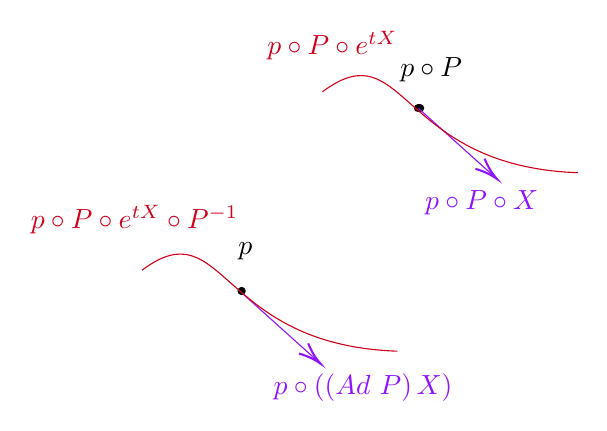
\begin{tikzpicture}[x=0.75pt,y=0.75pt,yscale=-1,xscale=1]
%uncomment if require: \path (0,255); %set diagram left start at 0, and has height of 255

%Shape: Free Drawing [id:dp49245771404128114] 
\draw  [color={rgb, 255:red, 0; green, 0; blue, 0 }  ][line width=3] [line join = round][line cap = round] (316.8,160) .. controls (316.8,160) and (316.8,160) .. (316.8,160) ;
%Shape: Free Drawing [id:dp8730283138166564] 
\draw  [color={rgb, 255:red, 0; green, 0; blue, 0 }  ][line width=3] [line join = round][line cap = round] (401.8,72) .. controls (402.13,72) and (402.47,72) .. (402.8,72) ;
%Straight Lines [id:da0031941210242911744] 
\draw [color={rgb, 255:red, 144; green, 19; blue, 254 }  ,draw opacity=1 ]   (317,161) -- (353.31,193.66) ;
\draw [shift={(354.8,195)}, rotate = 221.97] [color={rgb, 255:red, 144; green, 19; blue, 254 }  ,draw opacity=1 ][line width=0.75]    (10.93,-3.29) .. controls (6.95,-1.4) and (3.31,-0.3) .. (0,0) .. controls (3.31,0.3) and (6.95,1.4) .. (10.93,3.29)   ;
%Straight Lines [id:da5503181757486022] 
\draw [color={rgb, 255:red, 144; green, 19; blue, 254 }  ,draw opacity=1 ]   (402,72) -- (438.31,104.66) ;
\draw [shift={(439.8,106)}, rotate = 221.97] [color={rgb, 255:red, 144; green, 19; blue, 254 }  ,draw opacity=1 ][line width=0.75]    (10.93,-3.29) .. controls (6.95,-1.4) and (3.31,-0.3) .. (0,0) .. controls (3.31,0.3) and (6.95,1.4) .. (10.93,3.29)   ;
%Curve Lines [id:da27326141828123984] 
\draw [color={rgb, 255:red, 208; green, 2; blue, 27 }  ,draw opacity=1 ]   (268.8,150) .. controls (308.8,120) and (304.8,186) .. (391.8,189) ;
%Curve Lines [id:da863373974756469] 
\draw [color={rgb, 255:red, 208; green, 2; blue, 27 }  ,draw opacity=1 ]   (355.8,64) .. controls (395.8,34) and (391.8,100) .. (478.8,103) ;

% Text Node
\draw (314,135.4) node [anchor=north west][inner sep=0.75pt]    {$p$};
% Text Node
\draw (392,46.4) node [anchor=north west][inner sep=0.75pt]    {$p\circ P$};
% Text Node
\draw (331,198.4) node [anchor=north west][inner sep=0.75pt]  [color={rgb, 255:red, 144; green, 19; blue, 254 }  ,opacity=1 ]  {$p\circ \left(\left(\text{Ad} \ P\right) X\right)$};
% Text Node
\draw (404,110.4) node [anchor=north west][inner sep=0.75pt]  [color={rgb, 255:red, 144; green, 19; blue, 254 }  ,opacity=1 ]  {$p\circ P\circ X$};
% Text Node
\draw (328,33.4) node [anchor=north west][inner sep=0.75pt]  [color={rgb, 255:red, 208; green, 2; blue, 27 }  ,opacity=1 ]  {$p\circ P\circ e^{tX}$};
% Text Node
\draw (214,117.4) node [anchor=north west][inner sep=0.75pt]  [color={rgb, 255:red, 208; green, 2; blue, 27 }  ,opacity=1 ]  {$p\circ P\circ e^{tX} \circ P^{-1}$};


\end{tikzpicture}\\

Dessa forma, vamos definir:

$$\Pi_p = \span \{ p  \circ (\Ad\ P) X : P \in \mathcal{P}, X \in \mathcal{F}\}$$

Esse será nosso candidato à espaço tangente $T_p \mathcal{O}_{p_0}$.

\begin{lemma}
    Para cada $p \in \mathcal{O}_{p_0}$, $\dim \Pi_p = \dim \Pi_{p_0}$
\end{lemma}

\dem Necessariamente existe $Q \in \mathcal{P}$ tal que $p = p_0 \circ Q$.
Considere o isomorfismo $dQ_{p_0}:T_{p_0}M \to T_p M$. Dado um elemento
arbitrário $p_0 \circ (\Ad P) X \in \Pi_{p_0}$, temos que:

$$dQ_{p_0}(p_0 \circ (\Ad P) X \in \Pi_{p_0}) = 
p_0 \circ P \circ X \circ P^{-1} \circ Q =$$
$$= p_0 \circ Q \circ Q^{-1} \circ P \circ X
\circ P^{-1} \circ Q = (p_0 \circ Q) \circ (\Ad(Q^{-1} \circ P) X) \in \Pi_p$$

E dessa forma, $dQ_{p_0}(\Pi_{p_0}) \subseteq \Pi_p$. Similarmente,
$d(Q^{-1})_p(\Pi_p) \subseteq \Pi_{p_0}$. Portanto, $\Pi_p$ e $\Pi_{p_0}$
tem a mesma dimensão. \qed\\

Introduzimos a notação:

$$(\Ad \mathcal{P})\mathcal{F} = \{(\Ad\ P) X : P \in \mathcal{P}, X \in \mathcal{F}\}$$\\

Vamos agora colocar uma topologia e estrutura suave em $\mathcal{O}_{p_0}$.

Seja $m = \dim \Pi_{p_0}$. Para um ponto arbitrário $p \in \mathcal{O}_{p_0}$,
sejam $V_1, \dots, V_m \in (\Ad \mathcal{P})\mathcal{F}$ tais que
$\{p \circ V_1, \dots, p \circ V_m\}$ seja uma base de $\Pi_p$. Introdizimos o mapa:

$$\psi_p : (t_1, \dots, t_m) \mapsto p \circ e^{t_1V_1} \circ \dots \circ e^{t_mV_m}$$

Primeiramente, demonstramos que a imagem de $\psi_p$ está contida em $\mathcal{O}_{p_0}$.
De fato, cada $V_i$ pode ser escrito como $V_i = (\Ad P_i) X_i$ para $P_i \in \mathcal{P}$
e $X_i \in \mathcal{F}$. Dessa forma:

$$e^{tV_i} = e^{t (\Ad P_i) X_i} = P_i \circ e^{t X_i} \circ P_i^{-1} \in \mathcal{P}$$

e portanto $\psi_p(t_1,\dots,t_m) \in \mathcal{O}_{p_0}$.

Como

$$\parti{\psi_p}{t_i}\bigg|_0 = q \circ V_i$$

$\psi_p|_O$ é uma imersão para uma vizinhaça $O \subseteq \real^m$ suficiente pequena
da origem.

Os conjuntos da forma $\psi_p(O)$,
onde $O$ é uma vizinhaça da origem tal que
$\psi_p|_O$ é uma imersão, são candidatos
à base de uma topologia em $\mathcal{O}_{p_0}$. Vamos demonstrar
algumas propriedades desses conjuntos:

\begin{itemize}
    \item Para $t \in O$, $(d\psi_p)_t(T_t \real^m) = \Pi_{\psi_p(t)}$.
    
    Como o posto de $\psi_p|_O$ é $m$ e $\dim \Pi_{\psi_p(t)} = m$, basta demonstrarmos
    que $\parti{\psi_p}{t_i}\bigg|_t \in \Pi_{\psi_p(t)}$. Temos que:

    $$\parti{\psi_p}{t_i}\bigg|_t =
    \parti{}{t_i}\bigg|_t p \circ e^{t_1V_1} \circ \dots \circ e^{t_mV_m} =
    p \circ e^{t_1V_1} \circ \dots\circ e^{t_iV_i}\circ V_i \circ e^{t_{i+1}V_{i+1}}\circ 
    \dots \circ e^{t_mV_m}=$$

    $$=p \circ e^{t_1V_1} \circ
    \dots\circ e^{t_mV_m} \circ e^{-t_m V_m}\circ \dots \circ e^{-t_{i+1}V_{i+1}}
    \circ V_i \circ e^{t_{i+1}V_{i+1}}\circ 
    \dots \circ e^{t_mV_m}$$

    Sendo $Q = e^{t_{i+1}V_{i+1}}\circ 
    \dots \circ e^{t_mV_m}$, temos:

    $$\parti{\psi_p}{t_i}\bigg|_t = \psi_p(t) \circ (\Ad Q^{-1})V_i \in \Pi_{\psi_p(t)}$$ \qed

    \item Os conjuntos da forma $\psi_p(O)$ formam uma base para uma topologia
    em $\mathcal{O}_{p_0}$. O espaço topológico gerado por essa base será denotado
    por $\mathcal{O}_{p_0}^\mathcal{F}$
    
    É sufiente demonstrarmos que dado $\psi_p(O)$
    e $p' \in \psi_p(O)$, para $O'$ pequeno o suficiente,
    $\psi_{p'}(O') \subseteq \psi_p(O)$

    Sejam $V_1', \dots, V_m'\in \mathcal{F}$ os campos tais que

    $$\psi_{p'}(t_1,\dots,t_m) = p' \circ e^{t_1V_1'} \circ \dots \circ e^{t_mV_m'}$$

    Considere primeiramente a curva $t_1 \mapsto p' \circ e^{t_1V_1'}$. Como
    para $t_1$ pequeno o suficiente
    sua velocidade $(p' \circ e^{t_1V_1'}) \circ V_1'$ pertence à
    $T_{p' \circ e^{t_1V_1'}} \psi_{p'}(O') =
    \Pi_{p' \circ e^{t_1V_1'}} = T_{p' \circ e^{t_1V_1'}} \psi_{p}(O)$,
    para $t_1$ pequeno o sufiente $(p' \circ e^{t_1V_1'}) \in \psi_{p}(O)$.

    Aplicando o mesmo argumento à curva
    $t_2 \mapsto p' \circ e^{t_1V_1'} \circ e^{t_2V_2'}$,
    obtemos que $p' \circ e^{t_1V_1'} \circ e^{t_2V_2'} \in \psi_{p}(O)$ para
    $t_1$ e $t_2$ pequenos o suficiente, e prosseguindo indutivamente,
    obtemos que $\psi_{p'}(t) \in \psi_{p}(O)$ para $t$ pequeno o suficiente. \qed

    \item A espaço $\mathcal{O}_{p_0}^\mathcal{F}$ é conexo.
    
    Basta notarmos que os mapas $t \mapsto p \circ e^{tX}$ são contínuos
    em$\mathcal{O}_{p_0}^\mathcal{F}$
    para $X \in \mathcal{F}$, e portanto quaisquer dois pontos de
    $\mathcal{O}_{p_0}^\mathcal{F}$ podem ser conectados por curvas contínuas
    e portanto $\mathcal{O}_{p_0}^\mathcal{F}$ é conexo.

\end{itemize}

Induzimos agora uma estrutura suave em $\mathcal{O}_{p_0}^\mathcal{F}$ declarando
os mapas $\psi_p|_O$ como cartas. Note que $T_p \mathcal{O}_{p_0}^\mathcal{F} = \Pi_p$.


Isso conclui a demonstração do Teorema de Órbita. \qed

\subsection{Folheações}
Considere uma partição $L = \{L_\alpha\}$ de $M$ em variedades conexas imersas.
As variedades imersas $L_\alpha$ são chamadas de folhas da partição,
e a folha que contém um ponto $p \in M$ é escrita como $L_p$.

\begin{definition}
    Uma partição $\{L_\alpha\}$ de $M$ em variedades conexas imersas
    é dita uma folheção singular se para cada $p \in M$ e cada vetor
    $v \in T_p L_p$, existe um campo $X \in \X(M)$ tangente as folhas da partição
    tal que $X_p = v$.
\end{definition}

\begin{definition}
    Uma folheação singular $\{L_\alpha\}$ é dita regular
    se todas as suas folhas possuem a mesma dimensão.
\end{definition}

\begin{theorem}
    As órbitas $\{\mathcal{O}_p\}$ de um sistema
    de controle $\mathcal{F}$ formam uma folheação singular.
\end{theorem}

\dem Sejam $V_1, \dots, V_m \in (\Ad \mathcal{P})\mathcal{F}$ tais que
$\{p \circ V_1, \dots, p \circ V_m\}$ seja uma base de $T_p\mathcal{O}_p$.
Então, qualquer $v \in T_p\mathcal{O}_p$ pode ser escrito como
$v = \dsum t_i (p \circ V_i)$.

Simplesmente defina o campo $X = \dsum t_i V_i$. Como cada
$V_i \in (\Ad \mathcal{P})\mathcal{F}$, para cada $q \in M$,
$X_q = \dsum t_i (q \circ V_i)\in T_q\mathcal{O}_q$. \qed

Dada uma folheação singular $L$, indicamos por $\X(L)$ o conjunto dos campos
em $M$ tangentes à folheação, ou seja:

$$\X(L) = \{X \in \X(M) : \forall p \in M, X_p \in T_pL_p\}$$

Podemos facilmente verificar, pontualmente, que $\X(L)$ é um $C^\infty(M)$-submódulo
de $\X(M)$:

\begin{proposition}
    $\X(L)$ é um $C^\infty(M)$-submódulo
    de $\X(M)$
\end{proposition}

\dem Sejam $X, Y \in \X(L)$, $f \in C^\infty(M)$. Temos que:

\begin{itemize}
    \item $(X+Y)_p = X_p + Y_p \in T_pL_p$
    \item $(fX)_p = f(p)X_p \in T_pL_p$
\end{itemize} \qed

Além disso, podemos demonstrar:

\begin{proposition}
    $\X(L)$ é uma subálgebra de Lie de $\X(M)$
\end{proposition}

\dem Tendo em vista a proposição anterior, basta demonstrarmos
que dados $X, Y \in \X(L)$, $[X,Y] \in \X(L)$.

Considere a família à $1$ parâmetro $t \mapsto (\Ad e^{tX}) Y$. Como
$e^{tX}$ preserva a folha onde estão os pontos (isto é,
$p \in L_\alpha \iff p\circ e^{tX} \in L_\alpha$),
para cada $p \in M$, $p \circ (\Ad e^{tX}) Y \in T_pL_p$,
e portanto:

$$\deri{}{t}\bigg|_{t=0} p \circ (\Ad e^{tX}) Y = p \circ (\ad X) Y = p \circ [X,Y] \in T_pL_p$$

Ou seja, $[X,Y] \in \X(L)$ \qed

Com isso, podemos fazer uma estimativa inferior do espaço tangente às órbitas
de um sistema de controle:

\begin{definition}
    Seja $\mathcal{F} \subseteq \X(M)$. Definimos
    $\Lie \mathcal{F}$ como sendo a menor subálgebra de Lie
    de $\X(M)$ que contenha $\mathcal{F}$ e também seja
    um $C^\infty(M)$-submódulo de $\X(M)$.
\end{definition}

Note que a definição acima está bem definida pois a intersecção
de uma família de subálgebras de Lie que também são $C^\infty(M)$-submódulos
de $\X(M)$ também é uma subálgebra de Lie e um $C^\infty(M)$-submódulo.

\begin{definition}
    $\Lie_p \mathcal{F} = \{X_p : X \in \Lie\mathcal{F}\} $
\end{definition}

Indicando por $\mathcal{O}$ a folheção de $M$ nas órbitas
de $\mathcal{F}$, é claro que $\Lie \mathcal{F} \subseteq \X(\mathcal{O})$.
Dessa forma, temos:

\begin{proposition}
    $\Lie_p\mathcal{F} \subseteq T_p\mathcal{O}_p$
\end{proposition}

\subsection{Uma melhor descrição de $T_p \mathcal{O}_p$} Existe um caso específico,
no qual famílias da campos analíticos são inclusas, onde podemos melhor descrever
o espaço tangente à uma órbita $T_p\mathcal{O}_p$. É o
caso das famílias localmente finitamente geradas. Vamos agora explorar este caso.

\begin{definition}
    Um $C^\infty(M)$-submódulo $\mathcal{V}\subseteq \X(M)$ é dito finitamente
    gerado se exitem campos $V_1,\dots,V_k$ tal que:

    $$\mathcal{V} = \{\sum a_i V_i : a_i \in C^\infty(M)\}$$

    O conjunto $V_1,\dots,V_k$ é dito um gerador de $\mathcal{V}$.
\end{definition}

\begin{proposition}
    Seja $\mathcal{V}\subseteq \X(M)$ um $C^\infty(M)$-submódulo
    finitamente gerado, e $X \in \X(M)$. Então,
    se para todo $V \in \mathcal{V}$, temos que:

    $$(\ad X)V \in \mathcal{V}$$

    Segue que:

    $$(\Ad e^{tX})V \in \mathcal{V}$$

    Para todo $V \in \mathcal{V}$, $t \in \real$.
\end{proposition}

\dem Seja $V_1, \dots, V_k$ um conjunto gerador de $\mathcal{V}$. Por hipótese, temos:

$$[X,V_i] = \sum a_{ij} V_j$$

É suficiente mostrarmos que para cada $1 \leq i \leq k$ e cada $t \in \real$,
temos que:

$$V_i(t) = (\Ad e^{tX}) V_i \in \mathcal{V}$$

Diferenciando $V_i(t)$, obtemos a seguinte equação diferencial:

$$\dot{V_i}(t) = (\Ad e^{tX}) [X,V_i] = \sum (\Ad e^{tX}) (a_{ij} V_j)
= \sum (e^{tX} a_{ij}) V_j(t)$$

Definindo $a_{ij}(t) = e^{tX} a_{ij}$, e avaliando num ponto $p \in M$:

$$\dot{(p\circ V_i)}(t) = \sum p(a_{ij}(t))(p \circ V_j(t))$$

Defina a matriz $A_p(t) = [p(a_{ij}(t))]$. Se $\Gamma_p(t) = [\gamma_{p,ij}(t)]$
é a solução da EDO:

$$\dot{\Gamma}_p = A_p(t) \Gamma_p$$
$$\Gamma_p(0) = \id$$

Então, como $p \mapsto A_p(t)$ é suave, $p \mapsto \Gamma_p(t)$ também é suave.
Ou seja, as funções $\gamma_{ij} : p \mapsto \gamma_{p,ij}$ são suaves.

Dessa forma, $V_i(t)$ pode ser escrito como:

$$V_i(t) = \sum \gamma_{ij}(t) V_i(0) = \sum \gamma_{ij} V_i \in \mathcal{V}$$ \qed

Vamos introduzir agora submódulos localmente finitamente gerados.

\begin{definition}
    Dada uma família $\mathcal{F} \subseteq \X(M)$, e $U \subseteq M$ um aberto,
    definimos:

    $$\mathcal{F}|_U = \{X|_U : X \in \mathcal{F}\} \subseteq \X(U)$$
\end{definition}

\begin{definition}
    Um $C^\infty(M)$-submódulo $\mathcal{V}\subseteq \X(M)$ é dito localmente
    finitamente
    gerado se para cada $p \in M$, existe uma vizinhaça aberta $U$ de $p$
    tal que $\mathcal{V}|_U$ é finitamente gerado.
\end{definition}

E demonstramos um análogo à proposição 4.3 para submódulos localmente finitamente gerados:

\begin{proposition}
    Seja $\mathcal{V}\subseteq \X(M)$ um $C^\infty(M)$-submódulo
    localmente finitamente gerado, e $X \in \X(M)$. Então,
    se para todo $V \in \mathcal{V}$, temos que:

    $$(\ad X)V \in \mathcal{V}$$

    Segue que:

    $$(\Ad e^{tX})V \in \mathcal{V}$$

    Para todo $V \in \mathcal{V}$, $t \in \real$.
\end{proposition}

\dem Seja $p \in M$, e $U$ uma vizinhaça de $p$ tal que $\mathcal{V}|_U$ é finitamente
gerado. Temos que, para cada $V \in \mathcal{V}$, $(\ad X|_U) V_U \in \mathcal{V}|_U$,
e portanto $(\Ad e^{tX|_U})V|_U \in \mathcal{V}|_U$. Como $p$ é arbitrário,
temos que $(\Ad e^{tX})V \in \mathcal{V}$ \qed

Por fim, estamos prontos para demonstrar:

\begin{theorem}
    Seja $\mathcal{F} \subseteq \X(M)$ uma família tal que $\Lie \mathcal{F}$ seja
    localmente finitamente gerada. Então:

    $$T_p\mathcal{O}_p = \Lie_p \mathcal{F}$$
\end{theorem}

\dem Note que por definição, para todo $X \in \mathcal{F}$, $Y \in \Lie \mathcal{F}$,
$(\ad X) Y \in \Lie \mathcal{F}$.

Dessa forma, $(\Ad e^{tX}) Y \in \Lie \mathcal{F}$.

Como

$$T_p\mathcal{O}_p= \span\{(\Ad e^{t_1X_1}\circ \dots \circ e^{t_kX_k}) Y : X_1,\dots,X_k, Y \in \mathcal{F} ; t_1,\dots,t_k \in \real\}$$,

temos que $T_p\mathcal{O}_p \subseteq \Lie_p\mathcal{F}$. Como
$\Lie_p\mathcal{F} \subseteq T_p\mathcal{O}_p$, temos que $\Lie_p\mathcal{F} = T_p\mathcal{O}_p$. \qed



\subsection{Integração de Distribuições} Como aplicação do Teorema da Órbita, derivamos
alguns teoremas para integração de distribuições: o Teorema de Frobenius (para distribuições regulares)
e o Teorema de Stefan-Sussmann (para distribuições singulares).

\begin{definition}
    Uma distribuição singular $\Delta$ consiste da escolha de um subespaço
$\Delta_p \subseteq T_p M$ para cada $p \in M$, de forma que para cada $p \in M$,
exista uma vizinhaça $U_p$ de $p$ e uma coleção de campos $X_1, \dots, X_k$
tal que, para $q \in U_p$, $\Delta_q = \span\{q\circ X_1,\dots,q \circ X_k\}$.
\end{definition}

\begin{definition}
    Uma distribuição singular $\Delta$ é dita regular de posto $k$ se
    cada $\Delta_p$ tem dimensão $k$.
\end{definition}

Dizemos que uma distribuição (singular) $\Delta$ é integrável
se existe uma folheação (singular) $L$ tal que, para todo
$p \in M$, $T_p L_p = \Delta_p$. Cada $L_p$ é dita uma variedade integral
de $\Delta$, e $L$ é dita uma folheação integral de $\Delta$.

Note que uma distribuição regular integrável sempre será integrada em uma
folheação regular. Existem exemplos bem simples de distribuições não integráveis
em dimensão baixa.

De maneira similar à folheações, indicamos por $\X(\Delta)$ os campos tangentes à
uma distribuição $\Delta$:

$$\X(\Delta) = \{X \in \X(M) : \forall p \in M, X_p \in \Delta_p\}$$

Ainda similarmente às folheações,
podemos facilmente verificar, pontualmente, que $\X(\Delta)$
é um $C^\infty(M)$-submódulo
de $\X(M)$:

\begin{proposition}
    $\X(\Delta)$ é um $C^\infty(M)$-submódulo
    de $\X(M)$
\end{proposition}

\dem Dados, $X,Y \in \X(\Delta)$ e $f \in C^\infty(M)$, basta verificarmos pontualmente:

\begin{itemize}
    \item $(X+Y)_p = X_p + Y_p \in \Delta_p$
    \item $(fX)_p = f(p) X_p \in \Delta_p$
\end{itemize} \qed

No entanto, diferentemente das folheações, $\X(\Delta)$ pode não ser
uma sub-álgebra de Lie de $\X(M)$.

\begin{definition}
    Uma distribuição $\Delta$ satisfaz a condição de Frobenius
    se $\X(\Delta)$ é uma sub-álgebra de Lie de $\X(M)$.
\end{definition}

Note que, se $\Delta$ é integrável, e $L$ é a folheação integral de $\Delta$,
então $\X(\Delta) = \X(L)$. Dessa forma, a condição de Frobenius é uma condição
necessária para a integrabilidade de uma distribuição.

O clássico Teorema de Frobenius diz que ela também é suficiente no caso regular:

\begin{theorem}[Teorema de Frobenius]
    Seja $\Delta$ uma distribuição regular. Então, $\Delta$ é integrável
    se e somente se $\Delta$ satisfaz a condição de Frobenius.
\end{theorem}

\dem Já vimos que se $\Delta$ é integrável então $\Delta$
satisfaz a condição de Frobenius.
Suponha que $\Delta$ satisfaz a condição de Frobenius.
Considere a família $\X(\Delta) \subseteq \X(M)$ como um sistema de controle
geométrico.
Então, $\Lie \X(\Delta) = \X(\Delta)$, e dessa forma
para cada $p \in M$, $\Lie_p \X(\Delta) = \Delta_p$.

Além disso, podemos demonstrar que $\X(\Delta)$ é localmente
finitamente gerada: dado $p \in M$ e $V \in \X(\Delta)$, seja $U$ uma vizinhaça
de $p$ tal que existam campos $X_1, \dots, X_k$ onde, para $q \in U$,
$\Delta_q = \span\{q\circ X_1, \dots, q\circ X_k\}$. Para cada $q\in U$,
existe únicos (são únicos
pois cada $\Delta_q$ tem dimensão $k$,
e temos que $k$ vetores que geram $\Delta_q$, ou seja,
eles formam uma base de $\Delta_q$) $f_i(q) \in \real$, $1 \leq i \leq k$, tais que
$q\circ V = \sum f_i(q) (q \circ X_i)$.

Como $V$ é suave e cada $X_i$ é suave, as funções $f_i:q \mapsto f_i(q)$ também são suaves.
Dessa forma $V|_U = \sum f_i X_i|_U$. Além disso, dadas quaisquer $k$ funções suaves
$g_1, \dots, g_k$, temos que $\sum g_i X_i|_U \in \X(\Delta)|_U$. Dessa forma,
$X_1, \dots, X_k$ são um conjunto gerador de $\X(\Delta)|_U$.

Como $\Lie \X(\Delta) = \X(\Delta)$ é localmente finitamente gerada, temos que
$T_p \mathcal{O}_p = \Lie_p \X(\Delta) = \Delta_p$, e portanto
$\mathcal{O}$ é uma folheação integral de $\Delta$. \qed

O Teorema de Frobenius não se sustenta quando $\Delta$ é uma distribuição singular:
a falha na demonstração acontece ao tentarmos achar as funções $f_i$ (é possível garantir
a existencia de tais funções mas não sua suavidade). Existem exemplos
de distribuições singulares satisfazendo a condição de Frobenius mas que não
são integráveis.

Dessa forma, para distribuições singulares, invocamos a descrição de
$T_p \mathcal{O}_p$ do Teorema da Órbita para fornecemos uma condição necessária
e suficiente para integrabilidade de distribuições.

Dado $P \in \Diff(M)$, denote por $\Delta_p \circ P = \{X_p \circ P : X_p \in \Delta_p\}$.

\begin{definition}
    Seja $X \in \X(M)$ e $\Delta$ uma distribuição singular. Então, dizemos
    que $\Delta$ é invariante com respeito a $X$ se,
    para todo $t \in \real$, $\Delta_p \circ e^{tX} \subseteq \Delta_{p \circ e^{tX}}$.
\end{definition}

\begin{theorem}[Teorema de Stefan-Sussmann]
    Seja $\Delta$ uma distribuição singular. Então, são equivalentes:

    \begin{itemize}
        \item $\Delta$ é invariante com respeito à todo $X \in \X(\Delta)$.
        \item $\Delta$ é integrável.
    \end{itemize}
\end{theorem}

\dem Primeiramente suponha que $\Delta$ é integrável, seja $L$ uma folheação integral
de $\Delta$ e $X \in \X(\Delta) = \X(L)$. Seja ainda $p \in M$. Como $e^{tX}$ mapeia
$L_p$ em $L_p$ (isto é, $e^{tX}(L_p) \subseteq L_p$), temos
que $d(e^{tX})_p (T_p L_p) \subseteq T_{e^{tX}(p)} L_p$, e portanto
$\Delta_p \circ e^{tX} \subseteq \Delta_{p \circ e^{tX}}$, ou seja,
$\Delta$ é invariante com respeito à $X$.

Agora suponha que $\Delta$ é invariante com respeito à todo $X \in \X(\Delta)$.
Sejam $X, Y \in \X(\Delta)$.
Como $p \circ (\Ad e^{tX}) Y = ((p \circ e^{tX}) \circ Y) \circ e^{-tX})$,
e $(p \circ e^{tX}) \circ Y \in \Delta_{p \circ e^{tX}}$, temos que
$p \circ (\Ad e^{tX}) Y \in \Delta_{p \circ e^{tX}\circ e^{-tX}}= \Delta_p$.

Considere a folheação $\mathcal{O}$ dada pelas órbitas de $\X(\Delta)$.
Como, para cada $p \in M$,

$$T_p \mathcal{O}_p = \{p \circ (\Ad e^{t_1 X_1} \circ \dots \circ e^{t_kX_k}) Y : X_1, \dots, X_k, Y \in \X(\Delta)\}$$

temos que $T_p \mathcal{O}_p \subseteq \Delta_p$. Como é claro que $\Delta_p \subseteq T_p \mathcal{O}_p$,
temos que $\mathcal{O}$ é uma folheação integral de $\Delta$. \qed